\documentclass{pluto}




 
\title{\bf Java学习笔记}                                                      % Supply information
\author{白水}                                                                % for the title page.
\date{\today}                                                               % Use current date. 

\begin{document}
\begin{titlepage}
    \begin{center}
        \vspace*{1cm}
        \Huge
        \textbf{学习笔记}
        \vspace{0.5cm}

        \vfill
        \large
            \textit{Java}
            \vfill
   
            \vfill
            
\includegraphics[width=0.1\textwidth]{logo.png}
    \end{center}
\end{titlepage}

\frontmatter                                                                % End of preamble, start of text.

\tableofcontents

\mainmatter

\part{Java基础知识}
\chapter{JVM}
\label{chap:jvm}




\chapter{控制流程}
\label{chap:control_flow}

\section{switch}

\textbf{Java}

只支持基本类型(byte,short,char,int)、Enum类型以及String, Character, Byte, Short和Integer类。

只支持常量表达式,case会进行整数范围验证。

\begin{lstlisting}[style=cjava,caption={swtich},label=useless]
    /*
    * 枚举类型
    */
    public enum Day {
        SUNDAY, MONDAY, TUESDAY, WEDNESDAY,
        THURSDAY, FRIDAY, SATURDAY 
    }

    /*
    * 星期判断
    * @param day
    */
    public static void switchTestWithEnum(Day day) {
    switch (day) {
        case MONDAY:
            System.out.println("Today is Mondays.");
            break;
        default:
            System.out.println("Today is ...");
            break;
        }
   }

    public static void switchTestWithCharacter(Character character) {
        switch (character) {
            case 'a':
                System.out.println("character is a");
                break;
            case 'b':
                System.out.println("character is b");
            default:
                System.out.println("nothing...");
        }
    }

    //调用
    switchTestWithEnum(Day.SUNDAY);
    switchTestWithCharacter(new Character('a'));
\end{lstlisting}


\textbf{PHP}

case 表达式可以是任何求值为简单类型的表达式,即整型或浮点数以及字符串。不能用数组或对象,除非它们被解除引用成为简单类型。

允许使用分号代替 case 语句后的冒号

case比较执行的是松散比较 ==

 \begin{lstlisting}[language=php,caption={php-swtich},label=useless]
    $beer = 'caseC';
    $a ='caseA';

    switch($beer)
    {
	    case $a;
		    echo "this is caseA";
		break;
	    case 'caseB';
		    echo "this is caseB";
		break;
	    case 'case'.'C':
	        echo "this is caseC";
	    break;
        default;
            echo 'Please make a new selection...';
        break;
    }
\end{lstlisting}
    

\chapter{字符串}
\label{chap:string}

    Strings are constant; their values cannot be changed after they are created.

\section{字符串对象}

String对象是不可改变的,具有恒定性。

每个String对象都有常量值。

字符串字面常量是对String类的示例的饮用。

在Java中String对象可以认为是char数组的延伸和进一步的封装。

\begin{noteblock}
    这里所说的char数组不是C语言意义上的字符型数组,而是大致类似于C语言中的 char* 指针。 \par
    \begin{lstlisting}[style=cjava]
    String str = "Java学习笔记"; 
    \end{lstlisting}
    \begin{lstlisting}[style=cjava]
    char* str = "Java学习笔记";
    \end{lstlisting}
\end{noteblock}

\begin{lstlisting}[style=cjava]

    public final class String implements java.io.Serializable, Comparable<String>, CharSequence {

    /** The value is used for character storage. */
    private final char value[];

    /*
    * @param  value             Array that is the source of characters
    * @param  offset            The initial offset
    * @param  count             The length
    *
    * @throws  IndexOutOfBoundsException
    *          If the {@code offset} and {@code count} arguments index
    *          characters outside the bounds of the {@code value} array
    */
    public String(char value[], int offset, int count) {
        if (offset < 0) {
            throw new StringIndexOutOfBoundsException(offset);
        }
        if (count <= 0) {
            if (count < 0) {
                throw new StringIndexOutOfBoundsException(count);
            }
            if (offset <= value.length) {
                this.value = "".value;
                return;
            }
        }
        // Note: offset or count might be near -1>>>1.
        if (offset > value.length - count) {
            throw new StringIndexOutOfBoundsException(offset + count);
        }
        this.value = Arrays.copyOfRange(value, offset, offset+count);
    }

    }

\end{lstlisting}

通过上面String类的实现代码可以发现String类和value数组都是final类型,这就保证了String对象的不变性。这种不变性可以带来极大的好处。

\begin{itemize}
    \item 保证对String对象的任意操作都不会改变原字符串
    \item 意味着操作字符串不会出现线程同步问题
    \item 成就了字符串驻留以及共享(常量池)
\end{itemize}



\section{字符串连接操作符 + }


如果字符串连接操作符运算的结果不是编译时的常量表达式,那么该操作符会隐式地创建新的String对象。


如果只有一个操作数表达式是String 类型,那么就会在另一个操作数上执行字符串转换以在运行时产生字符串。 
对于简单类型Java还可以通过直接将简单类型转换为字符串而优化掉包装器对象的创建。

\textcolor{codepurple}{+}操作字符在语法上是左结合。

例如:

\begin{lstlisting}[style=cjava]

    String first = 1 + 2 + "Java";
    String second = "Java" + 1 + 2;
    String three = "Java" + null;
    System.out.println(first);
    System.out.println(second);
    System.out.println(three);

    /** 
    * Output: 
    * 
    * 3Java
    * Java12
    * Javanull
    * 
    */

\end{lstlisting}


在字符串转换方面要特别注意引用类型转行。

如果该引用是null,那么它转换为字符串"null"。

如果其他引用类型,则调用其对象上的toString()方法;如果调用toString()方法的结果是null,那么就用字符串"null"代替。


\section{字符串常量池}




\section{StringBuilder}









https://tech.meituan.com/2014/03/06/in-depth-understanding-string-intern.html

















































\chapter{内部类}
\label{chap:inner_class}

可以将一个类的定义放在另一个类的定义内部,这就是内部类。

内部类的对象与制造它的外围对象(enclosing object)之间就有一种联系,它能访问其外围对象的所有成员,而不要任何特殊条件。
内部类还拥有其外围类的所有元素的访问权。


\section{.this和.new}




Anonymous Inner Class

It is an inner class without a name and for which only a single object is created.
An anonymous inner class can be useful when making an instance of an object with certain “extras” such as overloading methods of a class or interface, without having to actually subclass a class.


are mainly created in two ways:

. Class (abstract or concrete)
. interface

The syntax of an anonymous class expression is like the invocation of a constructor, except that there is a class definition contained in a block of code.
匿名类表达式的语法类似于调用构造函数,只是在代码块中包含了一个类定义。

匿名内部类的创建格式

\begin{lstlisting}[style=cjava]
    new class(arguments) | interface()
    {
        //匿名内部类的类体部分
    }
\end{lstlisting}

okHttp中匿名类示例

\begin{lstlisting}[style=cjava]
    public abstract class Internal {
        public abstract void addLenient(Headers.Builder builder, String line);
    }

    Internal.instance = new Internal() {
        @Override public void addLenient(Headers.Builder builder, String line) {
        builder.addLenient(line);
        }
    }
\end{lstlisting}


Difference between Normal/Regular class and Anonymous Inner class:

A normal class can implement any number of interfaces but anonymous inner class can implement only one interface at a time.
A regular class can extend a class and implement any number of interface simultaneously. But anonymous Inner class can extend a class or can implement an interface but not both at a time.
For regular/normal class, we can write any number of constructors but we cant write any constructor for anonymous Inner class because anonymous class does not have any name and while defining constructor class name and constructor name must be same.


\subsection{嵌套类}

将内部类声明为static,内部类对象与其外围类对象之间则没有联系。

1. 要创建嵌套类的对象,并不需要其外围类的对象。
2. 不能从嵌套类的对象中访问非静态的外围类对象。




\chapter{对象}

\label{chap:object}

\section{初始化}


静态初始化只有在对象被创建或者第一次访问静态数据时才会被初始化。

初始化的顺序时先静态对象(如果他们尚未因前面的对象创建过程而被初始化),而后才是“非静态”对象。

以Dog类为示例总结一下对象的创建过程:

1. 当首次创建类型为Dog的对象或者Dog类的静态方法/静态域首次被访问时,java解释器必须查找类路径,以定位Dog.class文件

2.然后载入Dog.class ,有关静态初始化的所有动作都会执行。因此,静态初始化只在Class对象首次加载的时候进行一次。按照顺序。

3. 当用new Dog() 创建对象的时候,首先将在堆上为Dog对象分配足够的存储空间。

4. 这块存储空间会被清零,这就自动将Dog对象中的所有基本类型数据都设置成了默认值(数字为0,boolean为false),而引用则被设置成null(例如String)

5. 执行所有出现于字段定义处的初始化动作

6. 执行构造器(会涉及到继承的问题)


总结


基类静态代码块、基类静态成员字段并列优先级,按照代码中出现先后顺序执行(只有第一次加载类时执行)

派生类静态代码块、派生类静态成员字段并列优先级,按照代码中出现先后顺序执行(只有第一次加载类时执行)

基类普通代码块、基类普通成员字段并列优先级,按照代码中出现先后顺序执行

基类构造函数

派生类普通代码块、派生类普通成员字段并列优先级,按照代码中出现顺序执行

派生类构造函数

\subsection{对象拷贝}

对象的拷贝分为 shallow copy 和 deep copy 。

shallow copy 既浅拷贝。




https://zhuanlan.zhihu.com/p/26964202

\href{https://zgxxx.github.io/2019/02/27/20190227/}{clone}

\href{https://howtodoinjava.com/java/cloning/a-guide-to-object-cloning-in-java/}{clone}

PHP与Java一样,对象的对象属性都只是引用拷贝.

php的拷贝是通过clone关键字实现。






static

在static方法的内部不允许调用非静态方法,可以在没有创建任何对象的前提下,仅仅通过类本身来调用static方法。


初始化

初始化顺序

在类的内部,变量定义的先后顺序决定了初始化的顺序。

变量的初始化会在任何方法(包括构造器)被调用前得到初始化。



\chapter{范型}

\label{chap:generics}

\section{基本概念}

范型实现了参数化类型的概念。

\section{范型类}


\section{范型方法}

\section{通配符类型}

函数式接口

关于函数式接口

如果一个接口只有一个抽象方法,那么该接口就是一个函数式接口

如果我们在某个接口上声明了FunctionalInterface注解,那么编译器就会按照函数式接口的定义来要求该接口

如果某个接口只有一个抽象方法,但我们并没有给该接口声明FunctionalInterface注解,那么编译器依旧会将该接口看作是函数式接口

\begin{lstlisting}[style=cjava]
    List<Integer> list = Arrays.asList(1,2,3,4,5);

    list.forEach(new Consumer<Integer>(){
        @Override
        public void accept(Integer integer){
            System.out.println(integer);
        }
    });
\end{lstlisting}

在java中Lambda表达式是对象,他们必须依附与一类特别的对象类型-函数式接口(functional interface)

That instances of functional interfaces can be created with lambda expressions, method references, or constructor references.

函数式接口的实例可以通过lambda表达式,方法引用和构造函数引用创建。


外部迭代和内部迭代

Java lambda表达式是一种匿名函数;它是没有声明的方法,即没有访问修饰符,返回值声明和名字。

lambda操作符: ->
lambda左边:接口中抽象方法的形参列表
lamdba右边:重写抽象方法的方法体


当只有一个参数,并且类型可推导时,圆括号()可省略。例如: a-> return a*a

lambda 表达式的主体可包含零条或多条语句

如果lambda表达式的主体只有一条语句,花括号{} 可省略。匿名函数的返回类型与该主体表达式一致

如果Lambda表达式的主体包含一条以上语句,则表达式必须包含在花括号{}中。匿名函数的返回类型与代码块的返回类型一致,若没有返回值则为空



Function<T, R>
 
BiFunction<T, U, R>



\chapter{异常处理}

\section{异常}

\label{chap:exception}

异常的抛出同其他对象的创建一样,将使用new在堆上创建异常对象。然后当前的执行路径(它不能继续执行下去)被终止,并且从当前环境中弹出对异常对象的引用。
此时异常处理机制接管程序,并开始寻找一个恰当的地方来继续执行程序。而这个恰当的地方就是“异常处理程序”。它的任务是将程序从错误状态中恢复,以使程序能
要么换一种方式运行,要么继续运行下去。

Throwable类是所有异常的基类。

//此处有类图

Throwable Error Exception RuntimeException 非RuntimeException




\section{异常说明}

异常说明使用附加关键字throws。



重抛异常会把异常抛给上一级环境中的异常处理程序。同一个try块的后续catch子句将被忽略。




\begin{lstlisting}[language=java]
    
/**
 * The {@code Throwable} class is the superclass of all errors and
 * exceptions in the Java language. Only objects that are instances of this
 * class (or one of its subclasses) are thrown by the Java Virtual Machine or
 * can be thrown by the Java {@code throw} statement. Similarly, only
 * this class or one of its subclasses can be the argument type in a
 * {@code catch} clause.
 *
 * For the purposes of compile-time checking of exceptions, {@code
 * Throwable} and any subclass of {@code Throwable} that is not also a
 * subclass of either {@link RuntimeException} or {@link Error} are
 * regarded as checked exceptions.
 *
 * <p>Instances of two subclasses, {@link java.lang.Error} and
 * {@link java.lang.Exception}, are conventionally used to indicate
 * that exceptional situations have occurred. Typically, these instances
 * are freshly created in the context of the exceptional situation so
 * as to include relevant information (such as stack trace data).
 *
 * <p>A throwable contains a snapshot of the execution stack of its
 * thread at the time it was created. It can also contain a message
 * string that gives more information about the error. Over time, a
 * throwable can {@linkplain Throwable#addSuppressed suppress} other
 * throwables from being propagated.  Finally, the throwable can also
 * contain a <i>cause</i>: another throwable that caused this
 * throwable to be constructed.  The recording of this causal information
 * is referred to as the <i>chained exception</i> facility, as the
 * cause can, itself, have a cause, and so on, leading to a "chain" of
 * exceptions, each caused by another.
 *
 * <p>One reason that a throwable may have a cause is that the class that
 * throws it is built atop a lower layered abstraction, and an operation on
 * the upper layer fails due to a failure in the lower layer.  It would be bad
 * design to let the throwable thrown by the lower layer propagate outward, as
 * it is generally unrelated to the abstraction provided by the upper layer.
 * Further, doing so would tie the API of the upper layer to the details of
 * its implementation, assuming the lower layer's exception was a checked
 * exception.  Throwing a "wrapped exception" (i.e., an exception containing a
 * cause) allows the upper layer to communicate the details of the failure to
 * its caller without incurring either of these shortcomings.  It preserves
 * the flexibility to change the implementation of the upper layer without
 * changing its API (in particular, the set of exceptions thrown by its
 * methods).
 *
 * <p>A second reason that a throwable may have a cause is that the method
 * that throws it must conform to a general-purpose interface that does not
 * permit the method to throw the cause directly.  For example, suppose
 * a persistent collection conforms to the {@link java.util.Collection
 * Collection} interface, and that its persistence is implemented atop
 * {@code java.io}.  Suppose the internals of the {@code add} method
 * can throw an {@link java.io.IOException IOException}.  The implementation
 * can communicate the details of the {@code IOException} to its caller
 * while conforming to the {@code Collection} interface by wrapping the
 * {@code IOException} in an appropriate unchecked exception.  (The
 * specification for the persistent collection should indicate that it is
 * capable of throwing such exceptions.)
 *
 * <p>A cause can be associated with a throwable in two ways: via a
 * constructor that takes the cause as an argument, or via the
 * {@link #initCause(Throwable)} method.  New throwable classes that
 * wish to allow causes to be associated with them should provide constructors
 * that take a cause and delegate (perhaps indirectly) to one of the
 * {@code Throwable} constructors that takes a cause.
 *
 * Because the {@code initCause} method is public, it allows a cause to be
 * associated with any throwable, even a "legacy throwable" whose
 * implementation predates the addition of the exception chaining mechanism to
 * {@code Throwable}.
 *
 * <p>By convention, class {@code Throwable} and its subclasses have two
 * constructors, one that takes no arguments and one that takes a
 * {@code String} argument that can be used to produce a detail message.
 * Further, those subclasses that might likely have a cause associated with
 * them should have two more constructors, one that takes a
 * {@code Throwable} (the cause), and one that takes a
 * {@code String} (the detail message) and a {@code Throwable} (the
 * cause).
 *
 * @author  unascribed
 * @author  Josh Bloch (Added exception chaining and programmatic access to
 *          stack trace in 1.4.)
 * @jls 11.2 Compile-Time Checking of Exceptions
 * @since JDK1.0
 */

\end{lstlisting}




\section{异常捕获}

try.catch.finally

Java7开始,可以在一个catch表达式中对多种类型异常进行合并捕获。

\begin{lstlisting}[language=java]
    public int getBinaryInt(String number) {
        int result = -1;
        result = result / 2;
        try {
            result = Integer.parseInt(number, 2);
        } catch (NumberFormatException | ArithmeticException e) {
                
        }

        return result;
    }
\end{lstlisting}



\chapter{线程}
\label{chap:thread}

\section{线程基础知识}

\subsection{线程状态}

JVM线程的状态定义在Thread.State枚举中。包括:

\begin{itemize}
    \item   NEW         新建
    \item   RUNNABLE    就绪
    \item   BLOCKED     阻塞 
    \item   WAITING     
    \item   TIMED\_WAITING
    \item   TERMINATED
\end{itemize}


\begin{figure}[H]
    \centering
    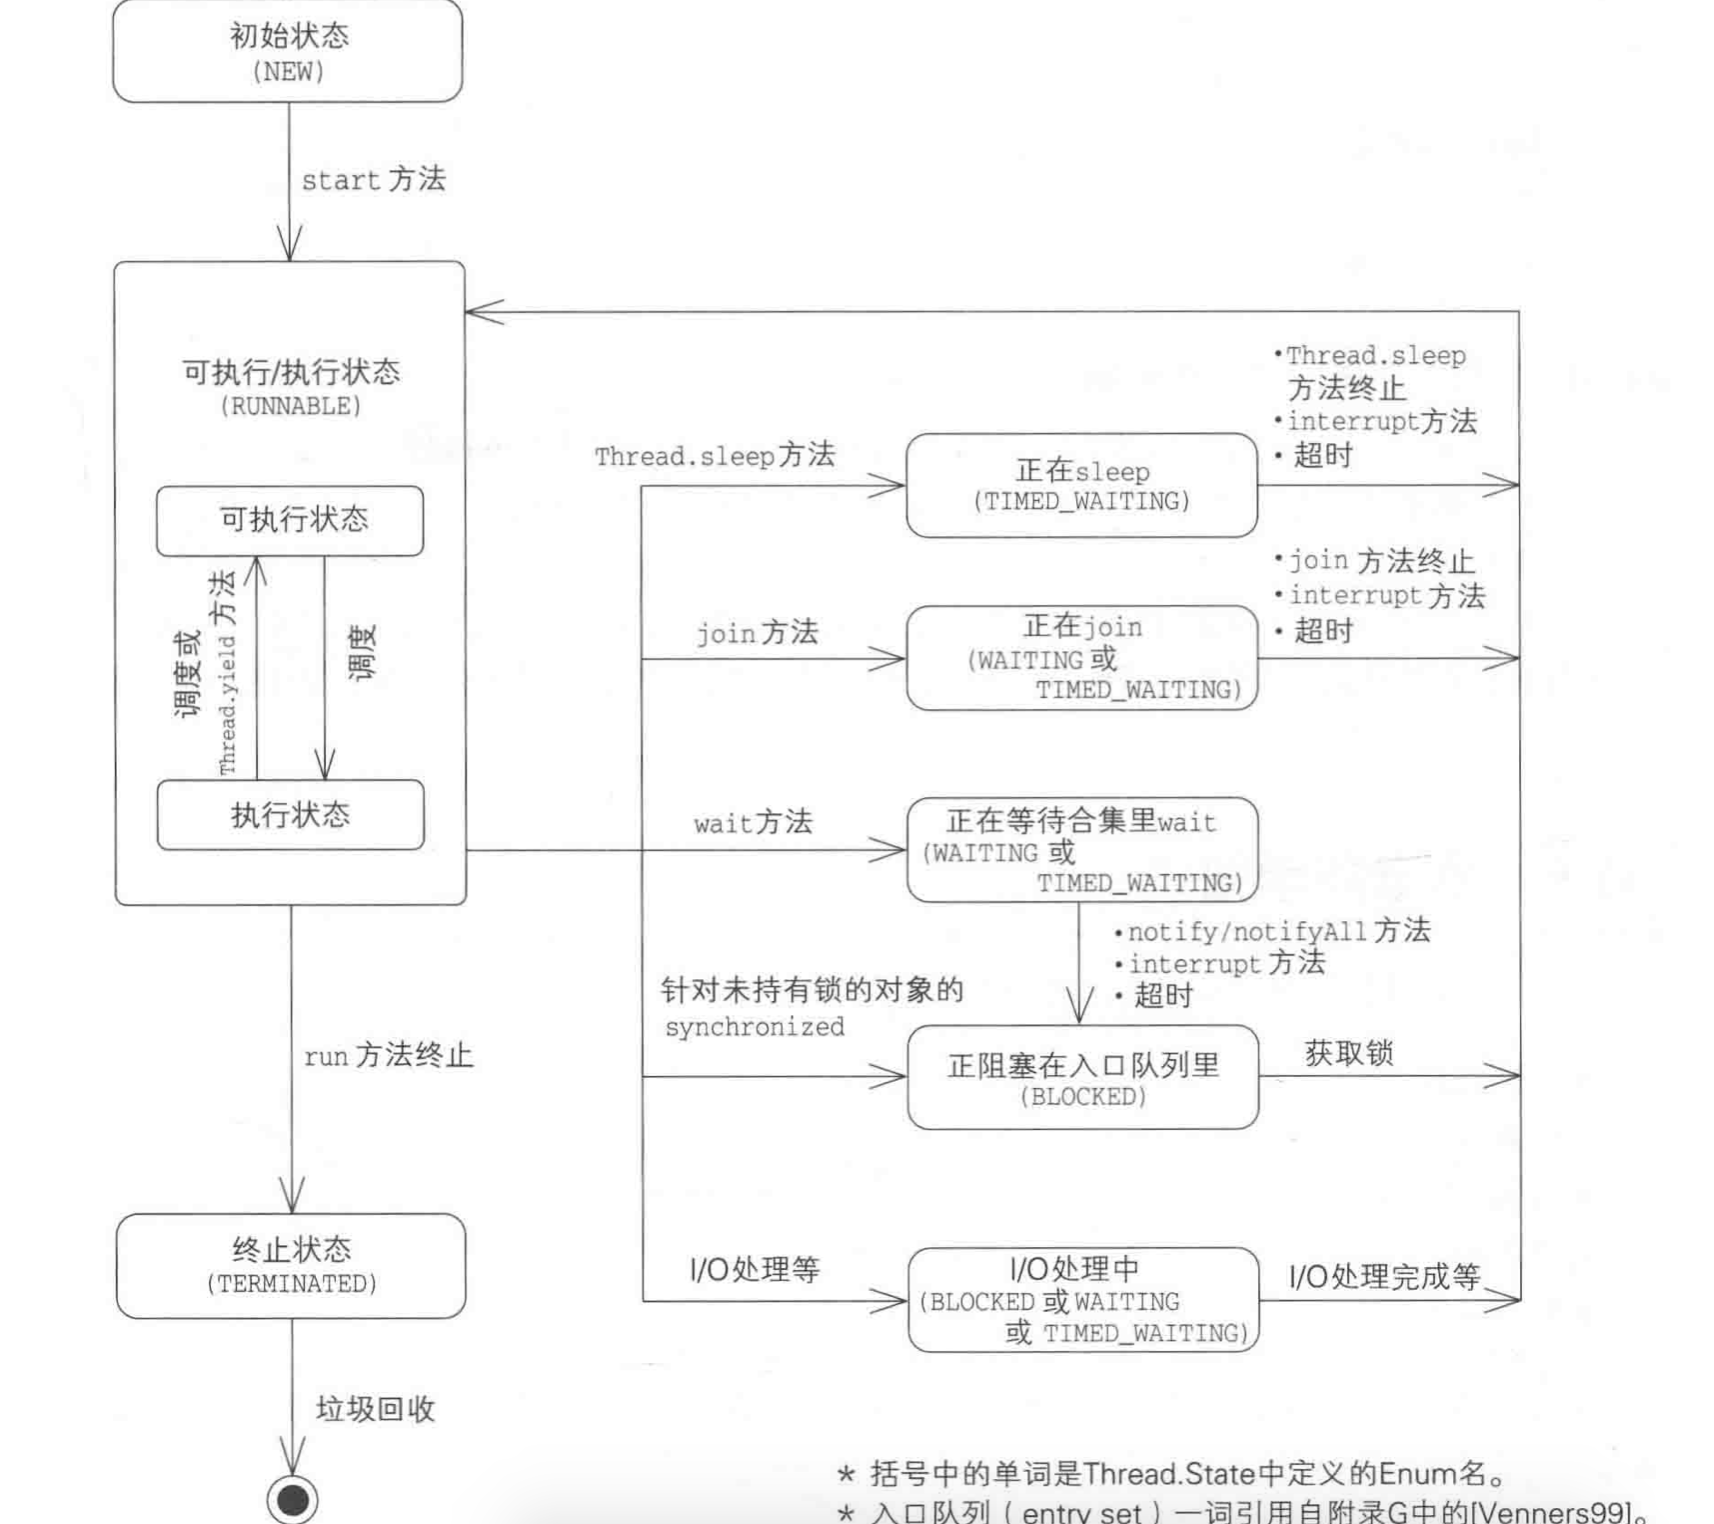
\includegraphics[width=1\textwidth]{thread/thread_states.png}
    \caption{线程状态迁移图(摘自《图解Java多线程设计模式》)}
\end{figure}

\subsubsection{NEW}

当线程被创建时,它只会短暂地处于这种状态。此时它已经分配了必须的系统资源,并执行了初始化。


\subsubsection{RUNNABLE}

只要调度器把时间片分配给线程,线程就可以运行。



下面为State枚举


\begin{lstlisting}[language=java]

public enum State {
        /**
         * 尚未启动的线程的线程状态
         */
        NEW,

        /**
         * 可运行线程的线程状态。 处于可运行状态的线程正在Java虚拟机中执行,
         * 但是它可能正在等待来自操作系统(例如处理器)的其他资源。
         */
        RUNNABLE,

        /**
         * 线程的阻塞状态,等待监视器锁定。
         * 处于阻塞状态的线程正在等待一个监视器锁进入一个同步块/方法,
         * 或者在调用Object.wait()后重新进入一个同步块/方法。
         */
        BLOCKED,

        /**
         * 等待线程状态
         * 一个线程由于调用下列方法之一而处于等待状态:
         * 
         *   Object.wait() 未超时
         *   Thread.join() 未超时
         *   LockSupport.park()
         * 
         * 处于等待状态的线程正在等待另一个线程执行特定的操作。
         * 例如: 一个线程在一个对象上已经调用了 Object.wait() ,并正在等待在另一个线程在另一对象上调用
         * Object.notify() or Object.notifyAll()。
         * 调用 thread.join() 的线程正在等待指定的线程终止。
         */
        WAITING,

        /**
         * 具有指定等待时间的等待线程的线程状态。
         * 线程处于定时等待状态,因为调用以下方法之一与指定的正等待时间:
         * 
         *   Thread.sleep()
         *   Object.wait(long)带超时参数
         *   Thread.join(long)带超时参数
         *   LockSupport.parkNanos
         *   LockSupport.parkUntil
         * 
         */
        TIMED_WAITING,

        /**
         * 终止状态。线程已经完成执行。
         */
        TERMINATED;
    }

\end{lstlisting}


\subsection{创建线程的方式}

创建线程的根本方法就是通过构造Thread类并且重写run()方法,然后调用start方法运行。

\begin{lstlisting}[language=java]

    public Thread();
    public Thread(String name);
    public Thread(ThreadGroup group, String name);

    public Thread(Runnable target);
    public Thread(Runnable target, String name);
    public Thread(ThreadGroup group, Runnable target, String name);
    public Thread(ThreadGroup group, Runnable target, String name, long stackSize);

\end{lstlisting}


创建线程有四种方式

\begin{itemize}
    \item  继承Thread类 
    \item  实现Runnable接口
    \item  实现Callable和Future接口
    \item  使用线程池方式
\end{itemize}


\subsubsection{实现Runnable接口}

Runnable接口

\begin{lstlisting}[language=java]

    @FunctionalInterface
    public interface Runnable {
        public abstract void run();
    }

\end{lstlisting}

\begin{lstlisting}[language=java]

public class HelloRunnable implements Runnable {

    public void run() {
        System.out.println("Hello from a thread!");
    }

    public static void main(String args[]) {
        (new Thread(new HelloRunnable())).start();
    }
}

\end{lstlisting}

\subsubsection{继承Thread类}

Thread类也继承了Runnable接口

\begin{lstlisting}[language=java]

    public class MyThread extends Thread {
        public void run() {
            System.out.println(Thread.currentThread().getName() + ": Run!!!");
        }
    
        public static void main(String[] args) {
            MyThread thread = new MyThread();
            thread.start();
        }
    }

\end{lstlisting}

\subsubsection{实现Callable和Future接口}

\begin{figure}[H]
    \centering
    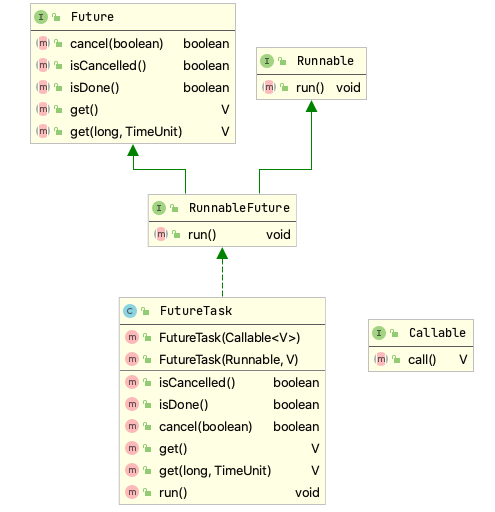
\includegraphics[width=0.8\textwidth]{thread/futuretask_diagram.png}
\end{figure}


\begin{lstlisting}[language=java]
    public class TaskWithResult implements Callable {

        private int id;
        public TaskWithResult(int id) {
            this.id = id;
        }

        @Override
        public Object call() throws Exception {
            return "Result of TaskWithResult is: " + id;
        }
    }

    public class FutureAndCallable {
    public static void main(String[] args) throws ExecutionException, InterruptedException {
        //不推荐使用Executors
        ExecutorService executorService = Executors.newCachedThreadPool();
        List<Future<String>> result = new ArrayList<>();
        for (int i = 0; i < 10; i++) {
            result.add(executorService.submit(new TaskWithResult(i)));
        }

        for (Future<String> future : result) {
            System.out.println(future.get());
        }

        executorService.shutdown();
    }
}



\end{lstlisting}


\subsubsection{使用线程池方式}

\begin{figure}[H]
    \centering
    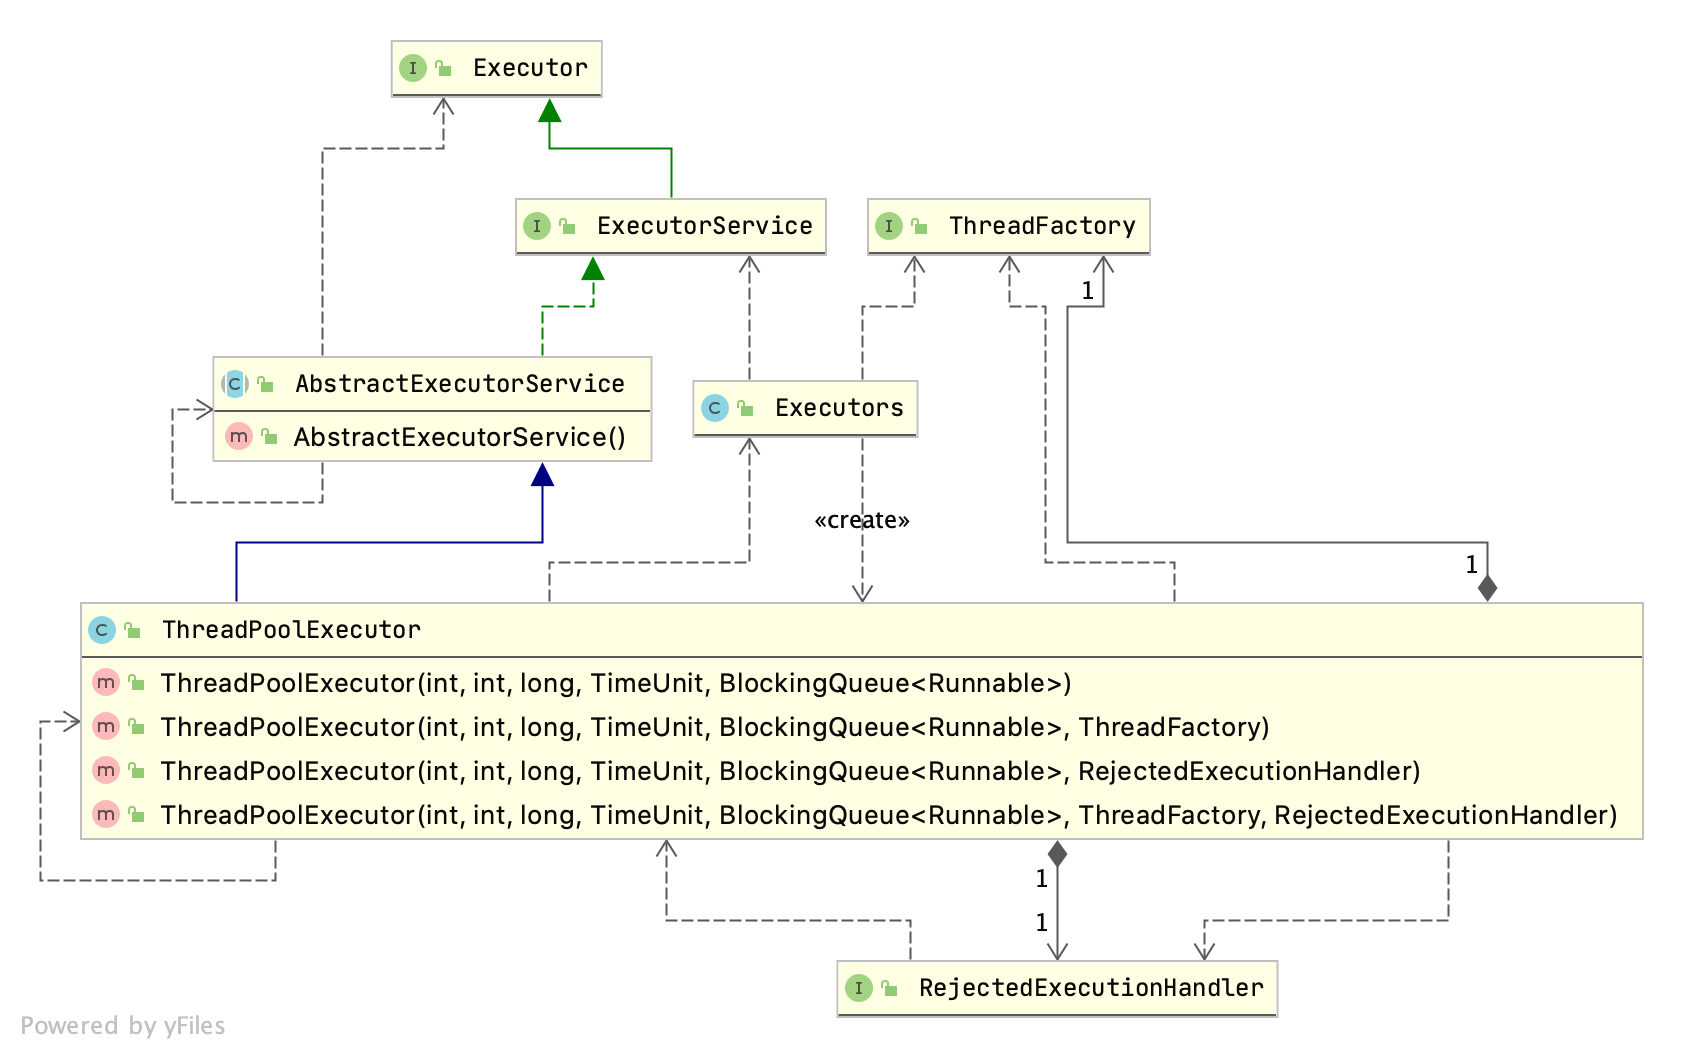
\includegraphics[width=1\textwidth]{thread/executor_diagram.png}
\end{figure}

线程池不允许使用 Executors 去创建,而是通过 ThreadPoolExecutor 的方式,这样的处理方式让写的同学更加明确线程池的运行规则,规避资源耗尽的风险。

Executors提供了如下线程池

\begin{itemize}
    \item newSingleThreadExecutor
    \item newFixedThreadPool
    \item newCachedThreadPool
    \item newScheduledThreadPool
    \item newSingleThreadScheduledExecutor
    \item newWorkStealingPool
\end{itemize}

\notebox{
    FixedThreadPool和SingleThreadExecutor:\newline
    运行的请求队列长度为Integer.MAX\_VALUE,可能会堆积大量的请求,从而导致OOM。

    CachedThreadPool:\newline
    允许的创建线程数为Integer.MAX\_VALUE,可能会创建大量的线程,从而导致OOM。
}

\begin{lstlisting}[language=java]
// 不推荐
ExecutorService executorService = Executors.newCachedThreadPool();

for (int i = 0; i < 5; i++) {
    executorService.execute(()->{
        System.out.println("Hello from a thread!");
    });
}

executorService.shutdown();

//推荐;指定最大线程数以及列队数
ExecutorService executor = new ThreadPoolExecutor(5, 5, 10L, TimeUnit.MILLISECONDS, new LinkedBlockingQueue<>(10));
for (int i = 0; i < 10; i++) {
    executor.execute(() -> System.out.println(Thread.currentThread().getName() + ":ThreadPoolExecutor"));
}

executor.shutdown();

\end{lstlisting}


\subsection{捕获异常}

不能捕获从线程中逃逸的异常。一旦异常跳出任务的run()方法,它就会向外传播到控制台。

可通过重写UncaughtExceptionHandler实现。使用setUncaughtExceptionHandler或者setDefaultUncaughtExceptionHandler方法。



\subsection{常用函数}

\begin{itemize}
    \item wait
    \item sleep
    \item join
    \item yield
    \item notify
    \item notifyAll
    \item interrupt
\end{itemize}


\subsubsection{wait}
调用wait()会释放对象上的锁。 

wait() 有两种形式。

第一种接受毫秒数做为参数,指“在此期间暂停”

在wait()期间对象锁是释放的
可以通过notify(),notifyAll()或者令时间到期,从wait()中恢复执行。

第二种不接受任何参数

wait()无限等待下去,直到线程接收到notify()或者notifyAll()的消息。

\subsubsection{sleep}
 调用sleep()的时候锁并不会被释放。

 \subsubsection{yield}
 yield()的时候锁并不会被释放。

\subsubsection{join}


wait(),notify(),notifyAll()是基类Object的一部分,而不是属于Thread的一部分。
只能在同步控制方法或者同步控制块里调用这三个方法,调用他们必须获取对象的锁。

为防止错失信号

\begin{lstlisting}[language=java]

    synchronized(sharedMonitor){
        while(someCondition){
            shareMonitor.wait();
        }
    }

\end{lstlisting}



\subsection{终止}

I/O和在synchronized块上的等待是不可中断的。















Hibernate

mybatis


\chapter{JVM}
\label{chap:jvm}




\section{javap命令}
\label{chap:javac}

Reads Java class and interface definitions and compiles them into bytecode and class files.

\begin{lstlisting}[language=cshell]
    
\end{lstlisting}
\section{javap命令}
\label{chap:tools_javap}

use the javap command to disassemble one or more class files.

\begin{lstlisting}[language=cshell]

用法: javap <options> <classes>

  -version                 版本信息
  -v  -verbose             输出附加信息
  -l                       输出行号和本地变量表
  -public                  仅显示公共类和成员
  -protected               显示受保护的/公共类和成员
  -package                 显示程序包/受保护的/公共类和成员 (默认)
  -p  -private             显示所有类和成员
  -c                       对代码进行反汇编
  -s                       输出内部类型签名
  -sysinfo                 显示正在处理的类的系统信息 (路径, 大小, 日期, MD5 散列)
  -constants               显示最终常量
  -classpath <path>        指定查找用户类文件的位置
  -cp <path>               指定查找用户类文件的位置
  -bootclasspath <path>    覆盖引导类文件的位置

\end{lstlisting}

示例:

\begin{lstlisting}[language=java]

javap -c Main.class

\end{lstlisting}

\subsection{Java字节码} 

Instruction set 


instructions fall into a number of broad groups:

\begin{itemize}
    \item 加载和存储指令(Load and store)(e.g. aload\_0, istore)
    \item 算术与逻辑指令(Arithmetic and logic) (e.g. ladd, fcmpl)
    \item 类型转换指令(Type conversion) (e.g. i2b, d2i)
    \item 对象创建与操作指令(Object creation and manipulation) (new, putfield)
    \item 堆栈操作指令(Operand stack management) (e.g. swap, dup2)
    \item 控制转移指令(Control transfer) (e.g. ifeq, goto)
    \item 方法调用与返回指令(Method invocation and return) (e.g. invokespecial, areturn)
\end{itemize}

大多数的指令有前缀和(或)后缀来表明其操作数的类型。如下表:

Many instructions have prefixes and/or suffixes referring to the types of operands they operate on.

\begin{table}[H]
    \centering
    \caption{前缀/后缀类型对照表}
    \begin{tabular}{|l|l|}
    \hline
    Prefix/suffix & Operand type    \\ \hline
    i           & integer           \\ \hline
    l           & long             \\ \hline
    s           & short             \\ \hline
    b           & byte              \\ \hline
    c           & character         \\ \hline
    f           & float             \\ \hline
    d           & double            \\ \hline
    a           & reference         \\ \hline
    \end{tabular}
    \end{table}


Java bytecode

\begin{table}[H]
    \centering
    \caption{Java字节码}
    \begin{tabular}{|l|l|l|}
    \hline
    mnemonic    & stack [before]->[after]   & description                                           \\ \hline
    aload\_0    & → objectref               & load a reference onto the stack from local variable 0  \\ \hline
    \end{tabular}
    \end{table}


        
\href{https://en.wikipedia.org/wiki/Java_bytecode_instruction_listings}{bytecode}

\href{http://blog.jamesdbloom.com/JavaCodeToByteCode_PartOne.html}{code}

\href{https://docs.oracle.com/javase/specs/jvms/se8/html/jvms-4.html#jvms-4.10.1.9}{jvms}
  
\section{java命令}
\label{chap:tools_java}

Launches a Java application.

\begin{lstlisting}[language=cshell]

    java [options] classname [args]

    java [options] -jar filename [args]

\end{lstlisting}

通过启动JRE来调用指定的类,调用此类的main()方法。
\begin{lstlisting}[language=Java]
    public static void main(String[] args)
\end{lstlisting}

\subsection{选项} 


\begin{itemize}
    \item   标准选项
    \item   非标准选项 
    \item   高级运行时选项      (Advanced Runtime Options)
    \item   高级JIT编译器选项   (Advanced JIT Compiler Options)
    \item   高级可维护性选项    (Advanced Serviceability Options)
    \item   高级垃圾收集选项    (Advanced Garbage Collection Options)
\end{itemize}



\subsubsection{标准选项} 

Java虚拟机(JVM)的所有实现都保证支持的标准选项。


* -agentlib:libname[=options]

加载指定的本机代理库。在库名之后,可以使用特定于库的以逗号分隔的选项列表。

如果指定 -agentlib:foo 选项,则JVM尝试加载位于由系统环境变量名为LD\_LIBRARY\_PATH(在OS X系统下变量名为 DYLD\_LIBRARY\_PATH)指定位置下的libfoo.so的库。

下面的示例将展示如何加载堆分析工具(HPROF)库,并且获取堆栈深度为3,每20msCPU的简单采样信息:

\begin{lstlisting}[language=cshell]

    -agentlib:hprof=cpu=samples,interval=20,depth=3

\end{lstlisting}  

下面这个示例将展示如何加载Java调试线协议库并且监听8000端口的套接字连接,在主类加载之前挂起JVM:


\begin{lstlisting}[language=cshell]

    -agentlib:jdwp=transport=dt_socket,server=y,address=8000

\end{lstlisting} 





\-XX:+PrintStringTableStatistics



\section{jps命令}
\label{chap:tools_jps}

Lists the instrumented Java Virtual Machines (JVMs) on the target system. 

只适用于HotSpot虚拟机。

\begin{lstlisting}[language=cshell]

jps [ options ] [ hostid ]

\end{lstlisting}

hostid可以是进程的标识符或者类似于URL的 [protocol:][[//]hostname][:port][/servername] 地址

如果jps命令没有指定hostid参数,那么工具只搜索本机运行的JVM。如果指定了hostid,那么他将通过指定的地址来搜索JVM。
使用指定hostid的主机必须运行着jstatd进程。

\subsection{选项} 

\menlo{-q}

只输出JVM标识符的列表,不输出类名、JAR文件名以及传递给main方法的参数。


\menlo{-m}

输出传递给mian方法的参数。嵌入式JVMS可能输出为空。


\menlo{-l}

输出应用程序主类的完整包名或应用程序JAR文件的完整路径名。

\menlo{-v}

输出传递给JVM的参数。

\menlo{-V}

只输出本地JVM标识符,不输出类名、JAR文件以及传递给main方法的参数。


\menlo{-Joption}

将选项传递给JVM,其中的选项是Java应用程序启动程序参考页面中描述的选项之一。例如,-J-Xms48m将启动内存设置为48 MB。



输出格式:

\begin{lstlisting}[language=cshell]

lvmid [ [ classname | JARfilename | "Unknown"] [ arg* ] [ jvmarg* ] ]

\end{lstlisting}



示例:

\begin{lstlisting}[language=cshell]
jps

    18027 Java2Demo.JAR
    18032 jps
    18005 jstat

\end{lstlisting}


\begin{lstlisting}[language=cshell]

jps -m remote.domain:2002

       3002 /opt/jdk1.7.0/demo/jfc/Java2D/Java2Demo.JAR
       3102 sun.tools.jstatd.jstatd -p 2002

    \end{lstlisting}
\section{jcmd命令}
\label{chap:tools_jcmd}

Sends diagnostic command requests to a running Java Virtual Machine (JVM).

\begin{lstlisting}[language=cshell]

    jcmd [-l|-h|-help]

    jcmd pid|main-class PerfCounter.print

    jcmd pid|main-class -f filename

    jcmd pid|main-class command[ arguments]

\end{lstlisting}


jcmd工具向JVM发送诊断命令请求。必须在当前运行着JVM机器上执行,并且具有与JVM具有相同的user和group标识。

运行jcmd不带参数或者使用 \-l 选项时,相当于jps (\textcolor[rgb]{0,0,1}{\ref{chap:tools_jps}}),会输出java进程标识符。

如果将进程标识符(pid)或主类(main-class)作为第一个参数,则jcmd将诊断命令请求发送给具有指定标识符或发具有指定main-class名称的Java进程。

如果使用0作为进程标识符,则会将诊断命令请求发送给所有可用的Java进程。


* Perfcounter.print

打印指定Java进程可用的性能计数器。性能计数器的列表可能因Java进程而异。


* -f filename

从文件中读取诊断命令。文件中每个命令必须单独一行。以\# 开头的命令会被忽略。如果命令行中包含\textcolor{codepurple}{stop}关键字则结束命令行读取。

* command [arguments]

要发送到指定Java进程的命令。可以通过向该进程发送\textcolor{codepurple}{help}命令来获得给定进程的可用诊断命令列表。

如果参数中包含空格,则必须使用单引号或者双引号扩起来。注意使用转义字符($\backslash$)转义单/双引号。


\begin{lstlisting}[language=cshell]

   jcmd 15 help     # 15为java进程id

    #### output ####

    15:
    The following commands are available:
    JFR.stop
    JFR.start
    JFR.dump
    JFR.check
    VM.native_memory
    VM.check_commercial_features
    VM.unlock_commercial_features
    ManagementAgent.stop
    ManagementAgent.start_local
    ManagementAgent.start
    VM.classloader_stats
    GC.rotate_log
    Thread.print
    GC.class_stats
    GC.class_histogram
    GC.heap_dump
    GC.finalizer_info
    GC.heap_info
    GC.run_finalization
    GC.run
    VM.uptime
    VM.dynlibs
    VM.flags
    VM.system_properties
    VM.command_line
    VM.version
    help

\end{lstlisting}

\begin{lstlisting}[language=cshell]
    jcmd 15 help GC.heap_info
\end{lstlisting}








\chapter{内存模型}
\label{chap:memory}

\section{Java内存模型与线程}
 
\begin{figure}[H]
    \centering
    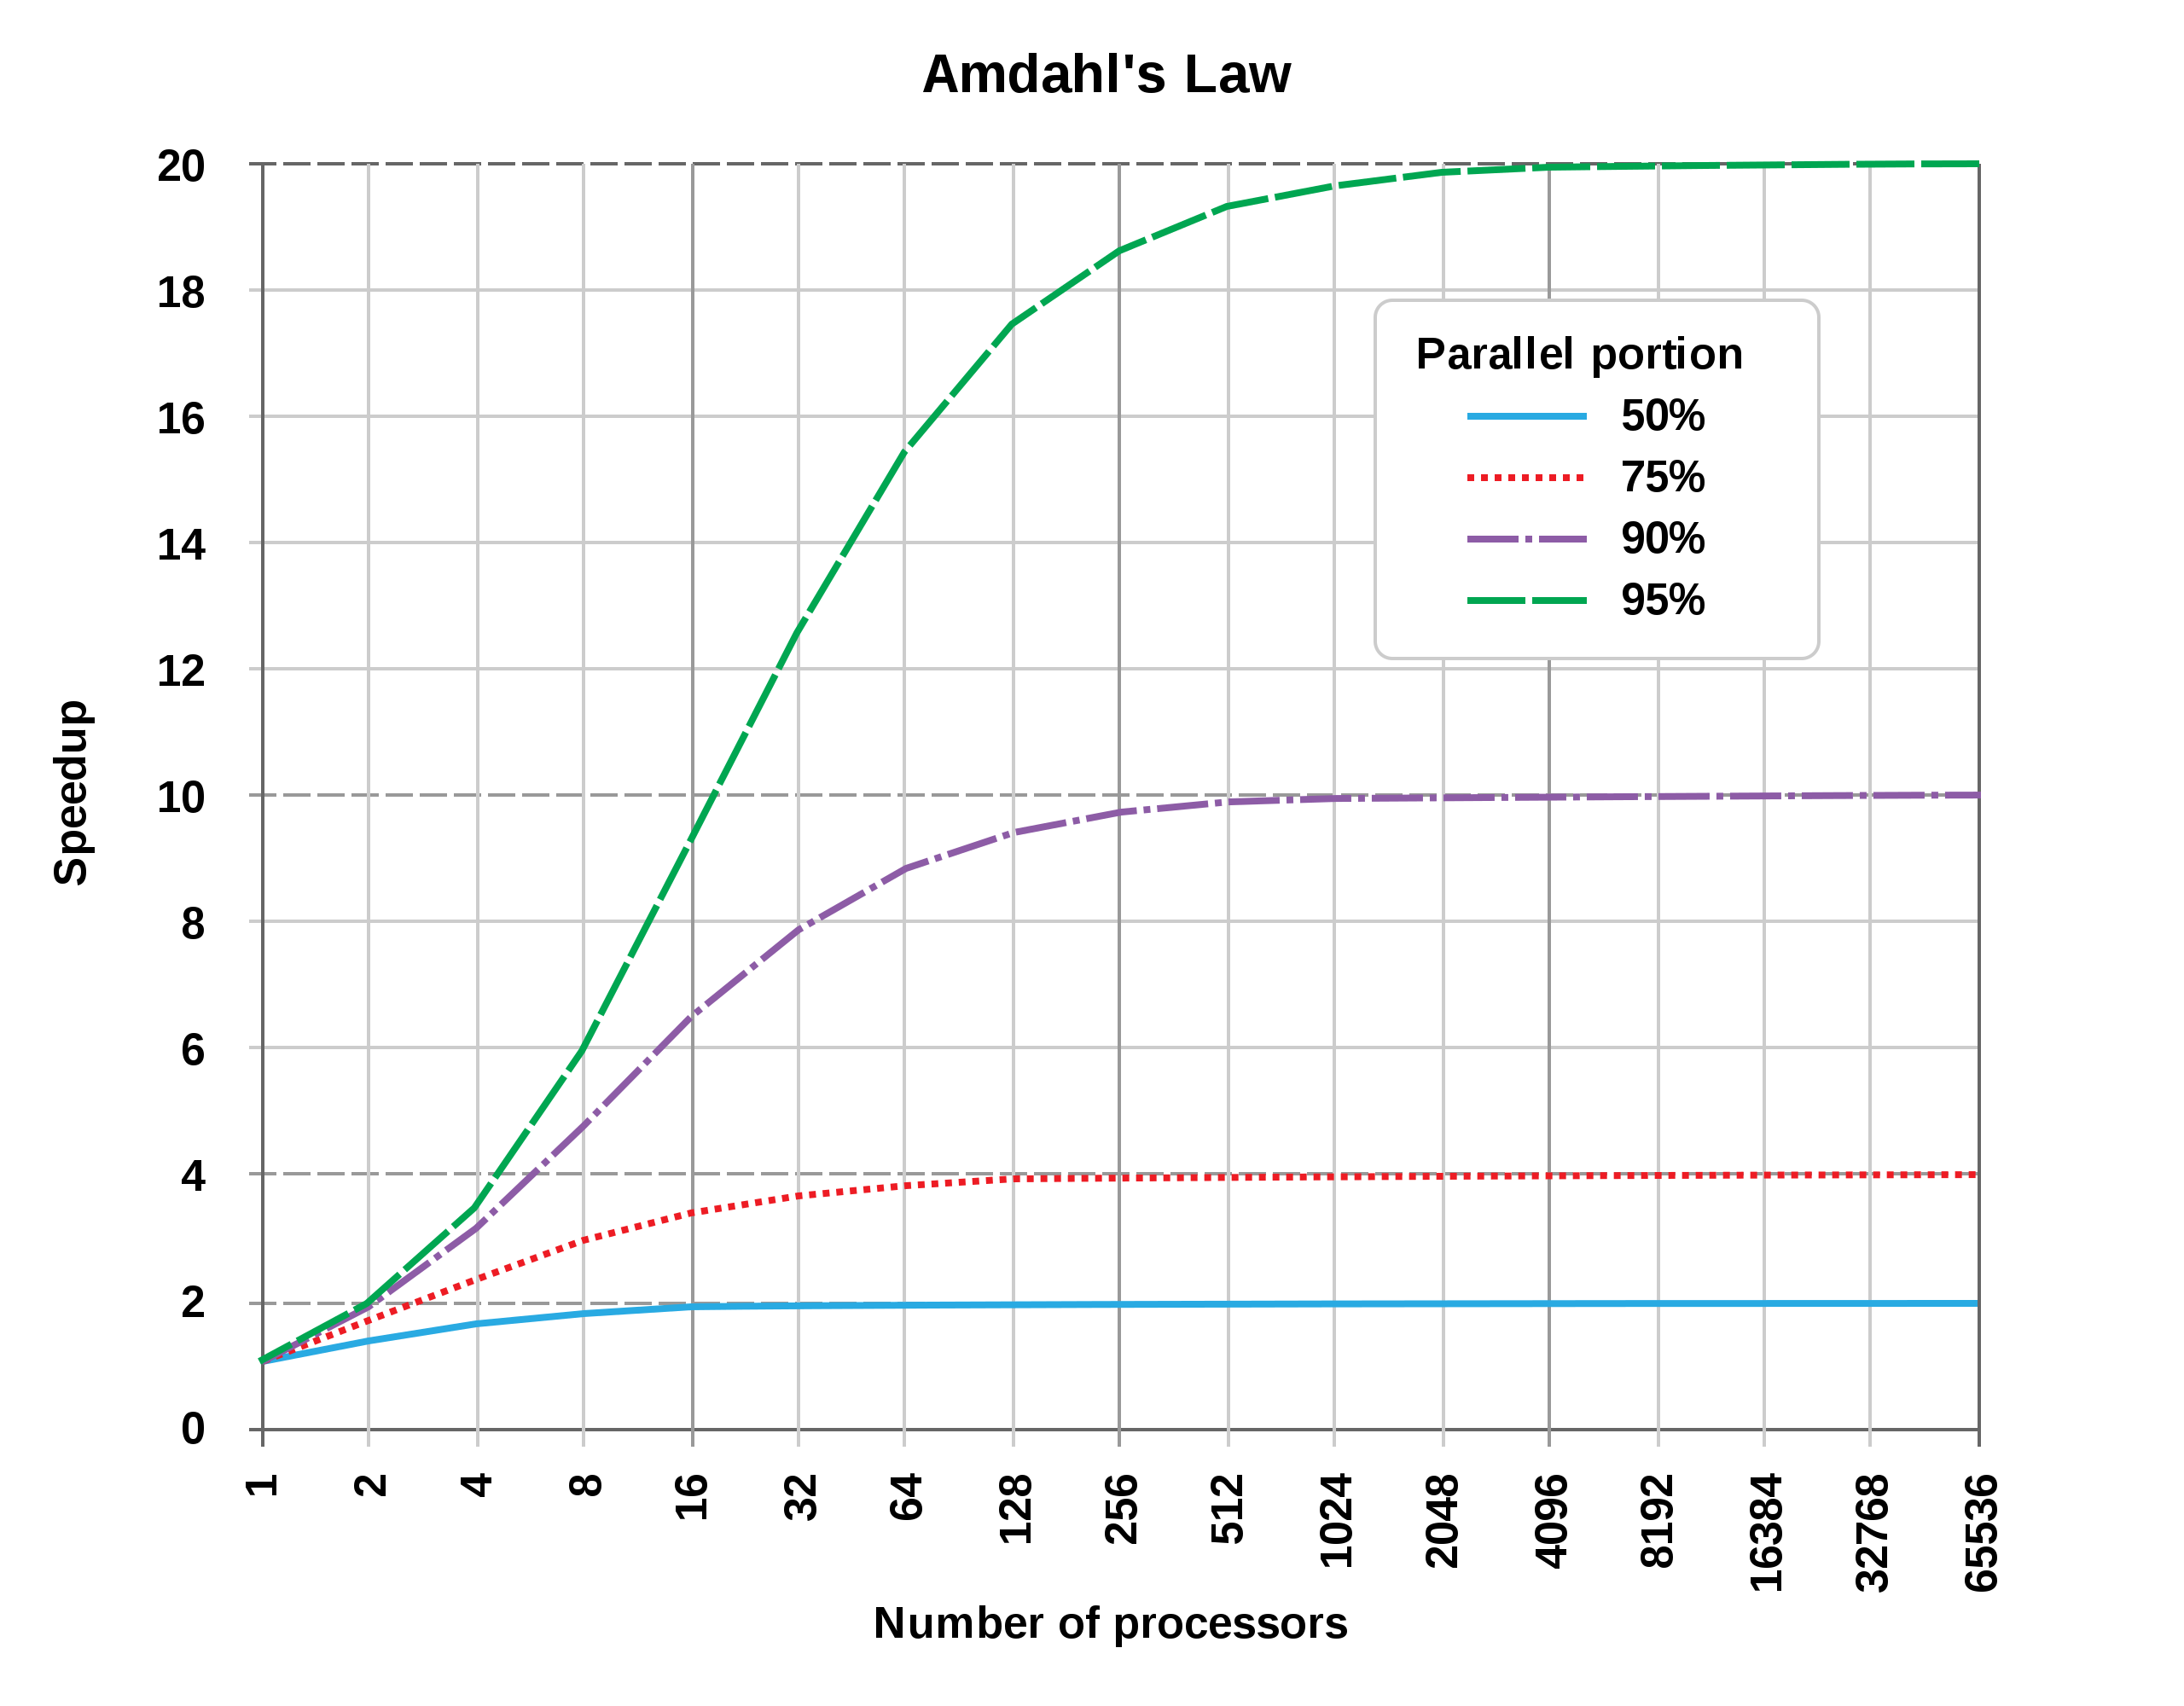
\includegraphics[width=0.8\textwidth]{parallel/amdahls-law-0.png}
    \caption{Amdahl's Law 阿姆达尔定律}
\end{figure}

并发不得不知的阿姆达定律。

一个程序(或者一个算法)可以按照是否可以被并行化分为下面两个部分:

\begin{itemize}
    \item 可以被并行化的部分
    \item 不可以被并行化的部分 
\end{itemize}


程序串行执行的总时间我们记为\textbf{T}。

时间\textbf{T}包括:不可以被并行和可以被并行部分的时间。不可以并行的部分记为\textbf{B}, 可以被并行的部分就是\textbf{T} - \textbf{B}。即 \textbf{T} = \textbf{B} + (\textbf{T} – \textbf{B}) 

定义如下:

\begin{lstlisting}

 T = 串行执行的总时间

 B = 不可以并行的总时间

 T - B = 并行部分的总时间

\end{lstlisting}


\textbf{T} - \textbf{B} 是可并行化的部分,以并行的方式执行可以提高程序的执行速度。可以提速多少取决于有多少线程或者多少个CPU来执行。线程或者CPU的个数我们记为\textbf{N}。可并行化部分被执行的最快时间可以通过下面的公式计算出来:

(\textbf{T} – \textbf{B} ) / \textbf{N} 或 (1/\textbf{N}) * (\textbf{T} - \textbf{B})

根据阿姆达定律,当可并行部分使用`N`个线程或CPU执行时,程序的总执行时间为:

\textbf{T}(\textbf{N}) = \textbf{B} + (\textbf{T} - \textbf{B}) / \textbf{N}

\notebox{T(N)表示并行因子为N的总执行时间。T(1)就是并行因子为1时的总执行时间。 T(N) = B + (T(1) – B) / N }


示例

\begin{lstlisting}
/*
 * 总时间为1。串行时间为0.4,那么并行时间为0.6。
 */

// 并行因子为2时
T(2) = 0.4 + ( 1 - 0.4 ) / 2
 = 0.4 + 0.6 / 2
 = 0.4 + 0.3
 = 0.7

// 并行因子为5时
 T(5) = 0.4 + ( 1 - 0.4 ) / 5
 = 0.4 + 0.6 / 6
 = 0.4 + 0.12
 = 0.52
\end{lstlisting}

图示

并行因子分别为1,2,3时。

\begin{figure}[H]
    \centering
    \subfigure[并行因子=1]{
        \label{P1}
        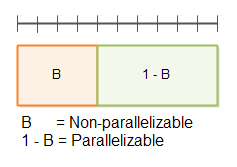
\includegraphics[width=0.45\textwidth]{parallel/amdahls-law-1.png}}
    \subfigure[并行因子=2]{
        \label{P2}
        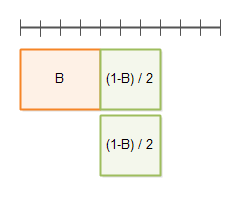
\includegraphics[width=0.45\textwidth]{parallel/amdahls-law-2.png}}
        \caption{并行因子分别为1,2时}
\end{figure}

\begin{figure}[H]
    \centering
    \label{P3}
    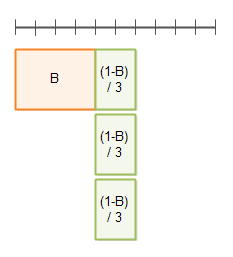
\includegraphics[width=0.8\textwidth]{parallel/amdahls-law-3.png}
    \caption{并行因子=3}
\end{figure}


\subsubsection{定义} 

并行计算中的\textbf{加速比}是用并行前的执行速度和并行后的执行速度之比来表示的,它表示了在并行化之后的效率提升情况。


 \begin{figure}[H]
    \centering
    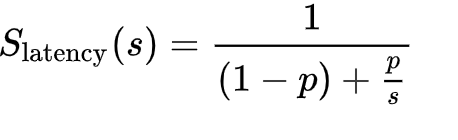
\includegraphics[width=1\textwidth]{parallel/amdahls-definition.png}
    \caption{阿姆达尔定律}
\end{figure}

S(latency)代表理论上的加速比

s 为并行处理结点个数

p 为并行计算部分所占比例

1-p为串行计算部分所占比例

这样:

当p = 1时,最大加速比p = s,

当p = 0时,最小加速比S = 1,

当 s→∞ 时,极限加速比S→ 1/(1-p),这也就是加速比的上限。

例如,若加速前并行代码执行时间占整个代码的执行时间的75%(p=0.75),则加速后并行处理的总体性能的提升不可能超过原先的4倍。

因此可以推断出:

 \begin{figure}[H]
    \centering
    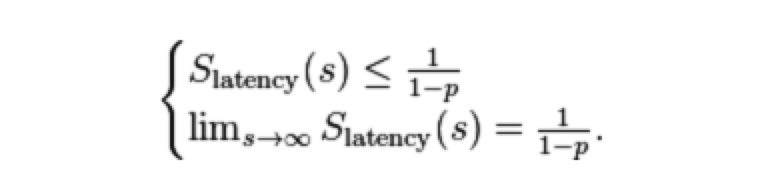
\includegraphics[width=1\textwidth]{parallel/amdahls-definition-1.png}
    \caption{阿姆达尔定律}
\end{figure}

阿姆达尔定律强调:当串行换比例一定时,加速比是有上限的,不管你堆叠多少个CPU参与计算,都不能突破这个上限。


\subsection{Gustafson's law 古斯塔夫森定律}


 \begin{figure}[H]
    \centering
    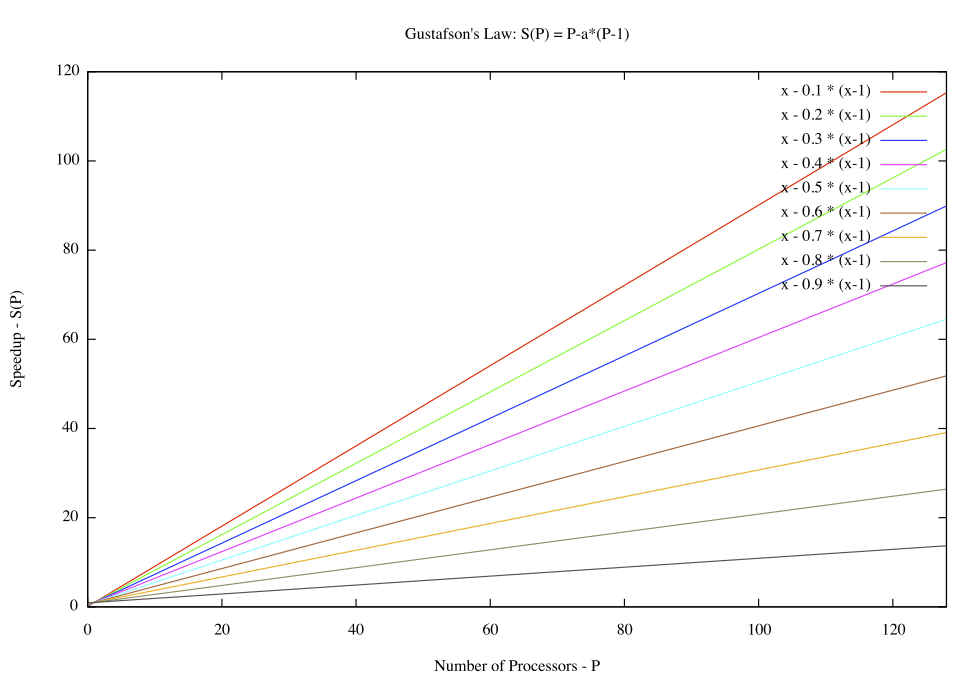
\includegraphics[width=1\textwidth]{parallel/gustafson.png}
    \caption{古斯塔夫森定律}
\end{figure}

 \begin{figure}[H]
    \centering
    
\includegraphics[width=1\textwidth]{parallel/gustafson-definition.png}
    \caption{古斯塔夫森定律定义}
\end{figure}

古斯塔夫森定律强调的是:如果可被并行化的代码所占比例足够大,那么加速比就能随着CPU的数量线性增长。



\subsection{JAVA内存模型 JMM}

JAVA内存模型 Java Memory Model JMM














\chapter{IPv6}

\section{基础知识}
\label{chap:ipv6_base}

\subsection{IPv6格式}

IPv6二进位制下为128位长度。




\subsection{问题}

 1. IP地址转为int实现


2. DNS域名解析中A、AAAA、CNAME、MX、NS、TXT、SRV、SOA、PTR各项记录的作用

https://blog.hackroad.com/operations-engineer/basics/13255.html

article, report, book und letter standard font size 

\begin{table}[]
    \begin{tabular}{|l|l|l|l|}
    \hline
                                    & \multicolumn{3}{l|}{standard font size} \\ \hline
    command                         &  10pt        & 11pt       & 12pt        \\ \hline
    \textbackslash{}tiny            &  5pt         & 6pt        & 6pt         \\ \hline
    \textbackslash{}scriptsize      &  7pt        &	 8pt	    & 8pt         \\ \hline
    \textbackslash{}footnotesize    &  8pt        &	 9pt	    & 10pt        \\ \hline
    \textbackslash{}small           &  9pt        &	 10pt       & 11pt        \\ \hline
    \textbackslash{}normalsize     &   10pt       &	 11pt       & 12pt        \\ \hline
    \textbackslash{}large          &   12pt       &	 12pt       & 14pt        \\ \hline
    \textbackslash{}Large          &   14pt       &	 14pt       & 17pt        \\ \hline
    \textbackslash{}LARGE    	   &   17pt       &	 17pt       & 20pt        \\ \hline
    \textbackslash{}huge           &   20pt       &	 20pt       & 25pt        \\ \hline
    \textbackslash{}Huge           &   25pt       &	 25pt       & 25pt        \\ \hline
    \end{tabular}
    \end{table}




%\\newpage 分页命令


%\\par:分段

\end{document}                                                            % The required last line
